\documentclass{article}
\usepackage{multicol}
\usepackage{graphicx}
\begin{document}
\title{class 12 probality}
\maketitle
\LARGE
\begin{enumerate}
\item If $\mathrm{A}$ and $\mathrm{B}$ are two events such that $\Pr(A|B) = 2\Pr(B|A)$ and $\Pr(B) +\Pr(B)=\frac{2}{3}$ , then $\Pr(B)$ is equal to
\begin{multicols}{2}
\begin{enumerate}
\item $\frac{2}{9}$
\item $\frac{7}{9}$
\item $\frac{4}{9}$
\item $\frac{5}{9}$
\end{enumerate}
\end{multicols}
\item a) Two balls are drawn at random one by one with replacement from an urn containing equal number of red balls and green balls . Find the probability distribution of number of red balls.Also, find mean of random variable $$OR$$ b) A and B throw a die alternately till one of them gets a '$6$'and wins the game .Find their respective probabilities of winning, if A starts t he ga m e    f  i r  s  t m Recent studies suggest that roghly  $12\%$ of the world population is lefthanded.
\begin{figure}
\centering
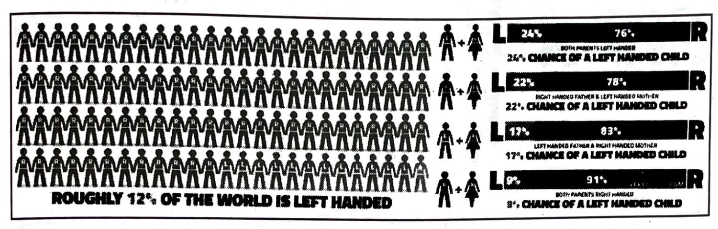
\includegraphics[width=\columnwidth]{left.png}
\end{figure}
Depending upon the parents,the chance of having a left handed child are follows:
\textbf{A}: When both father and mother are handed :
             chances of left handed child is $24\%$

\end{enumerate}
\end{document}



